\chapter{引言}\label{chap:fundamental}

近几十年来,在实际问题的驱动下,数学物理反问题已经成为应用数学领域中成长的最快的领域之一。这得益于数学物理反问题在石油勘探、遥感技术、医疗成像、信号处理以及雷达散射成像等众多科学技术领域当中的广泛应用。地球物理反问题是数学物理反问题中比较活跃的分支之一,其基本思想是通过对观测数据进行分析,来预测或估计地下介质的几何结构和物理参数信息。散射问题以声波、电磁波以及弹性波三类波动方程为模型来解释波在介质中传播的各种物理现象,而与之相对应的逆散射问题则在地球物理反问题的科学研究和实际应用中起到至关重要的作用。逆散射问题应用价值较大,但又具有强非线性和高度不适定性的特性,于是关于逆散射问题的理论研究和数值重构算法非常富有挑战性和吸引力。在众多应用数学家的努力下,很多难点被攻克,尤其是以全空间为背景模型的散射问题和逆散射问题研究。然而,在勘探地球物理反问题当中,欲探寻的目标距离地表较远,且地下大多是分层介质的复杂结构,于是以全空间为数学模型有时并不能对实际问题做到很好地刻画。故而本文在前人研究的基础上,对一般半空间以及半空间分层介质上的散射问题和逆散射问题加以研究,特别是考虑如何从数值上构造高效稳定的成像重构算法。在本章,我们将首先简单介绍一下声波半空间上的散射问题和逆散射问题,然后再介绍两种常见的波导结构以及相应的散射问题和逆散射问题。
\section{声波半空间散射问题与逆散射问题}
地球表面是一个特殊的分界面,它将介质划分为两个半空间,地面以上为空气介质,其密度与地面以下的岩石或者海平面以下的海水层相比可以忽略,故而以半空间为模型来研究散射问题和逆散射问题具有重要的应用价值。

令障碍物$D$为我们的成像目标,且$D$嵌入在背景介质速度为常数$c_0$的均匀半空间$\R^2_+$当中,其中$\R^2_+=\{(x_1,x_2)^T:x_1\in\R,x_2>0\}$. 我们假设$D$是一个有界的Lipschitz 区域,其边界记为 $\Gamma_D$. 若$D$为可穿透障碍物,则在半空间中,时谐声波波场$u(x,x_s)$满足如下Hemholtz方程和边界条件:
\begin{eqnarray}
 \Delta_x u(x,x_s)+k^2n(x)u(x,x_s)=-\delta_{x_s}(x),&in&\R^2_+   \label{into_p1_1}\\
 \frac{\partial u(x,x_s)}{\partial x_2}=0,&on&\Gamma_0  \label{into_p1_2}
\end{eqnarray}

其中$\omega$为频率,$k=\frac{\omega}{c_0}>0$为波数,$c(x)$表示波在介质中的传播速度以及$n(x)=\frac{c_0^2}{c^2(x)}$为折射系数的平方。此外,$x_s$为点源激发的位置,$\Gamma_0=\{(x_1,x_2)^T:x_1\in\R,x_2=0\}$表示半空间的边界。

为了保证方程\eqref{into_p1_1}-\eqref{into_p1_2}具有物理意义解的唯一性,$u(x,x_s)$在无穷远处需要满足著名的Sommerfeld辐射条件:
\begin{equation}\label{into_p1_3}
  \sqrt{r}\left(\frac{\partial u}{\partial r}-\i k u\right)\rightarrow0\ \ as\ \ r=|x|\rightarrow\infty
\end{equation}

令$N_k(x,y)$为满足如下方程的声波半空间Neumann格林函数:
\begin{eqnarray}
\left\{
\begin{array}{lll}
 \Delta_x N_k(x,y)+k^2N_k(x,y)=-\delta_{y}(x),&in&\R^2_+   \label{into_p2_1}\\
 & &\\
 \frac{\partial N_k(x,y)}{\partial x_2}=0,&on&\Gamma_0  \label{into_p2_2}\\
 & &\\
 \sqrt{r}\left(\frac{\partial N_k}{\partial r}-\i k N_k\right)\rightarrow0,&as&r=|x|\rightarrow\infty\label{into_p2_3}
\end{array}
\right.
\end{eqnarray}
直接验证可知
\begin{equation}
  N_k(x,y)=\Phi_{k}(x,y)+\Phi_{k}(x,y')
\end{equation}
其中$\Phi_k(x,y)=\frac{\i}{4}H_0^{(1)}(k|x-y|)$是波数为$k$的Hemholtz方程基本解,$y'=(y_1,-y_2)$ 是 $y=(y_1,y_2)\in\R^2_+$关于$\Gamma_0$的镜像点。


若令$u^i(x,x_s)$为在点源$x_s$处激发而产生的入射场,则$u^i(x,x_s)=N_k(x,x_s)$,从而散射场$u^s(x,x_s)=u(x,x_s)-u^i(x,x_s)$满足如下方程:
\begin{eqnarray}\label{half_scatter}
\left\{
\begin{array}{lll}
 \Delta u^s(x,x_s)+k^2u^s(x,x_s)=k^2[1-n(x)]u(x,x_s),&in&\R^2_+   \label{into_p3_1}\\
 & &\\
 \frac{\partial u^s(x,x_s)}{\partial x_2}=0,&on&\Gamma_0  \label{into_p3_2}\\
 & &\\
 \sqrt{r}\left(\frac{\partial u^s}{\partial r}-\i k u^s\right)\rightarrow0,&as&r=|x|\rightarrow\infty\label{into_p3_3}
\end{array}
\right.
\end{eqnarray}

类似地,我们可以考虑当散射体$D$为不可穿透障碍物时散射场所满足的方程。当障碍物不可穿透时,总场$u(x,x_s)$ 满足如下方程:
\begin{eqnarray}
\left\{
\begin{array}{lll}
 \Delta u(x,x_s)+k^2u(x,x_s)=-\delta_{x_s}(x),&in&\R^2_+\backslash\overline{D}   \label{into_p4_1}\\
 & &\\
 \frac{\partial u(x,x_s)}{\partial x_2}=0,&on&\Gamma_0  \label{into_p4_2}\\
 & &\\
 \sqrt{r}\left(\frac{\partial u}{\partial r}-\i k u\right)\rightarrow0,&as& r=|x|\rightarrow\infty\label{into_p4_3}
\end{array}
\right.
\end{eqnarray}

此外,我们还要对不同类型的不可穿透障碍物添加上合适的边界条件,具体如下:
\begin{itemize}
  \item 声软障碍物:
  \begin{equation}
     u=0,\ \ on\ \ \Gamma_D
  \end{equation}
  \item 声硬障碍物:
  \begin{equation}
    \frac{\partial u(x,x_s)}{\partial\nu}=0,\ \ on\ \ \Gamma_D
  \end{equation}
  \item 阻抗障碍物:
  \begin{equation}
    \frac{\partial u(x,x_s)}{\partial\nu}+\i k\eta(x)u(x,x_s)=0,\ \ on\ \ \Gamma_D
  \end{equation}
\end{itemize}
 这里$\eta(x)$为障碍物$D$的阻抗系数。

从而对于声软障碍物来说,散射场$u^s(x,x_s)=u(x,x_s)-u^i(x,x_s)$满足如下方程:
\begin{eqnarray}
\left\{
\begin{array}{lll}
 \Delta u^s(x,x_s)+k^2u^s(x,x_s)=0,&in&\R^2_+\backslash\overline{D}  \\
 & &\\
 \frac{\partial u^s(x,x_s)}{\partial x_2}=0,&on&\Gamma_0  \\
 & &\\
 u^s(x,x_s)=-N_k(x,x_s),& on&\Gamma_D\\
 & &\\
 \sqrt{r}\left(\frac{\partial u^s}{\partial r}-\i k u^s\right)\rightarrow0,&as&r=|x|\rightarrow\infty
\end{array}
\right.
\end{eqnarray}

对于声硬障碍物和阻抗障碍物,只须将在障碍物边界$\Gamma_D$上的边界条件分别换为
\begin{equation}
  \frac{\partial u^s(x,x_s)}{\partial\nu}=-\frac{\partial N_k(x,x_s)}{\partial\nu}
\end{equation}
和
\begin{equation}
  \frac{\partial u^s(x,x_s)}{\partial\nu}+\i k\eta(x)u^s(x,x_s)=-\left(\frac{\partial N_k(x,x_s)}{\partial\nu}+\i k\eta(x)N_k(x,x_s)\right)
\end{equation}
于是半空间散射问题即可定义如下:
\begin{question}[半空间散射问题]
$(i).$ 可穿透障碍物散射问题:
    已知障碍物位置、大小、形状和折射系数,求解散射场$u^s(x,x_s)$。\\
$(ii).$ 不可穿透障碍物散射问题:
    已知障碍物位置、大小、形状、边界类型和阻抗系数,求解散射场$u^s(x,x_s)$。
\end{question}

关于一般全空间声波散射问题的适定性的研究已经很完善,详见文献David Colton\cite{colton-kress,Cakoni2014A}和
William Mclean\cite{Mclean2000Strongly}。关于声波半空间散射问题适定性研究的文献也有很多,例如文献Zhang Bo\cite{Bo1998Acoustic},Simon N.Chandler-Wilde\cite{Chandler1996Scattering,Chandler1997The}。特别地,我们参考了
文献\cite{ch_ha}中关于声波半空间声软障碍物的适定性结果,其证明方法是利用经典的极限吸收原理,具体可参考文献
Rolf Leis\cite{Leis1986Initial}和Zhiming Chen\cite{cz2010,ch_cw}。


在本文中,我们主要对半空间上的逆散射问题感兴趣,特别是关于障碍物成像问题的数值重构算法。假设我们不知道障碍物的任何先验信息,包括障碍物是否可穿透以及$u(x,x_s)$在障碍物边界上所满足的边界条件,然后我们研究的问题具体如下:
 \begin{question}[半空间障碍物成像问题]\label{ques_half}
$(i).$   在远离障碍物的区域上采集散射数据$u^s(x,x_s)$或总场数据$u(x,x_s)$,通过数值重构算法确定出障碍物的位置、大小和形状。\\
$(ii).$  在远离障碍物的区域上采集无相位散射数据$|u^s(x,x_s)|$或总场数据$|u(x,x_s)|$,通过数值重构算法确定出障碍物的位置、大小和形状。
 \end{question}

 求解障碍物成像问题的方法主要分为两大类:直接成像法和迭代法。直接成像法主要是通过分析问题的本质特征,构造出一个直接成像函数,该函数通过对接收到的散射数据加以处理,可以直接对障碍物进行成像。具体而言,当采样点靠近障碍物边界时,成像函数呈现峰值;当采样点远离障碍物时,成像函数逐渐衰减,于是直接成像法不需要迭代求解正散射问题,就可以确定障碍物的位置、大小和形状。迭代法主要是将原始问题化成一个优化问题,通过建立目标函数,选取合适的数值优化算法,然后不断迭代来确定最优的参数,再代入原始问题。在一定条件下,迭代法能够较好地确定障碍物的位置和形状,甚至关于介质参数的定量信息。然而迭代法的收敛性和实用性却有待考量。首先,迭代法的收敛性分析极为复杂;其次,迭代法的收敛需要一个较好地初值,这就需要关于障碍物一定的先验信息;最后,由于迭代法每一步迭代都需要求解一个正散射问题,计算极为耗时,且十分依赖正散射问题的求解精度。因此,本文主要关注于如何构造求解障碍物成像问题的直接成像算法。特别地,我们主要研究了在实际当中应用广泛的一种直接成像算法,即逆时偏移成像算法。下面我们简单地对该算法做一个介绍。

%常见的迭代法和直接成像法介绍

\section{逆时偏移算法思想介绍}

逆时偏移成像算法(Reverse Time Migration)是一种直接成像法,由于其能够对复杂地质构造直接进行有效成像,因而在勘探地球物理反问题领域得到了广泛的应用,
%具体可参看文献
同时也引起了很多学者对其理论分析的研究
%,例如文献中基于高频渐进假设或者几何光学近似进行了渐进分析。
。文献Zhiming Chen\cite{cch_a}中,针对全空间时谐声波逆散射问题,首次提出了频率域单频逆时偏移成像算法,并且基于Hemholtz-Kirchhoff 恒等式,对成像函数建立了严格的分辨率分析。紧接着,他们在文献\cite{cch_e}中针对全空间电磁波逆散射问题,提出了新的单频电磁波逆时偏移算法;在文献\cite{ch_e}中针对全空间弹性波逆散射问题,提出新的单频弹性波逆时偏移算法,并且基于类似的Hemholtz-Kirchhoff恒等式,均建立了严格的分辨率分析。文献\cite{cch_a,cch_e,ch_e}分别针对声波、电磁波和弹性波逆散射问题提出的算法和理论构成了逆时偏移算法的数学理论基础。特别地,其所提算法的分辨率分析不需要高频渐进假设或几何光学近似,这是一个极大地进展。

在文献\cite{ch_cw}中,Zhiming Chen等人考虑了平板声波波导逆散射问题,提出了广义的Hemholtz-Kirchhoff恒等式,并以此为出发点构造了声波闭波导逆时偏移算法。然后他们在文献\cite{ch_ha}中对半空间时谐声波逆散射问题进行研究时,发现半空间模型下Hemholtz-Kirchhoff恒等式不再成立,于是其引入了点扩散函数,并通过对点扩散函数的分析建立了半空间声波逆时偏移算法的分辨率分析。
我们强调,点扩散函数的引入对于求解一般半空间模型以及半空间分层介质上的逆散射问题,有着至关重要的作用。

由于逆时偏移算法简单而有效、数值实现容易以及可扩展性较好,故而本文将从文献\cite{ch_ha}出发,继续对此算法进行研究。文献
\cite{ch_ha}中的算法主要是为解决问题\ref{ques_half}中的第一部分而提出的,算法所使用的的数据为散射场$u^s(x,x_s)$的所有信息。本文第二章将考虑对其加以改进以适用于问题\ref{ques_half}中的第二部分,使得改进后的算法仅需要利用总场的振幅信息即可。
逆时偏移算法的思想很简单,主要分为两步:计算反传播场和互相关关系,具体如下所示:
\begin{algorithm}
设$d>0$为孔穴半径,在$\Gamma_0^d:=\{(x_1,x_2);x_1\in(-d,d),x_2=0\}$上均匀分布着$N_s$个源点$x_s$和$N_r$个接收点$x_r$,其中
$s=1,2,\ldots,N_s;r=1,2,\ldots,N_r$。令$u^s(x_r,x_s)$为在接收点$x_r$处记录的由源点$x_s$激发而产生的散射场,以及区域$\Omega$为采样区域。然后对任意地$z\in\Omega$,计算反传播场和互相关关系:\\
$1^\circ$ 反传播: 对于 $s=1,\ldots,N_s$, 计算反传波场
\begin{equation}
  v_b(z,x_s)=\frac{|\Gamma_0^d|}{N_r}\sum\limits_{r=1}^{N_r}\frac{\partial\Phi_k(x_r,z)}{\partial x_2(x_r)}u^s(x_r,x_s),\  \  \forall z\in\Omega.
\end{equation}
$2^\circ$ 互相关: 对于 $z\in\Omega$, 计算成像函数
\begin{equation}
  I_d(z)=\Im\left\{\frac{|\Gamma_0^d|}{N_s}\sum\limits_{s=1}^{N_s}\frac{\partial\Phi_k(x_s,z)}{\partial x_2(x_s)}v_b(z,x_s)
  \right\}.
\end{equation}
将反传波场$v_b(z,x_s)$代入到成像函数$I_d(z)$,可得
\begin{equation}
  \qquad I_d(z)=\Im\left\{\frac{|\Gamma_0^d||\Gamma_0^d|}{N_sN_r}
  \sum\limits_{s=1}^{N_s}\sum\limits_{r=1}^{N_r}
  \frac{\partial\Phi_k(x_s,z)}{\partial x_2(x_s)}\frac{\partial\Phi_k(x_r,z)}{\partial x_2(x_r)}
  u^s(x_r,x_s)
  \right\},\  \ \forall z\in\Omega.\quad\quad
\end{equation}
若令$N_s,N_r\rightarrow\infty$,则上式可看做对如下积分的近似:
\begin{equation}
 \qquad  I_{\rm RTM}(z)=\Im\int_{\Gamma_0^d}\int_{\Gamma_0^d}\frac{\partial\Phi_k(x_s,z)}{\partial x_2(x_s)}\frac{\partial\Phi_k(x_r,z)}{\partial x_2(x_r)}
  u^s(x_r,x_s)ds(x_r)ds(x_s),\  \  \forall z\in\Omega.\quad\quad
\end{equation}
\end{algorithm}

与文献\cite{cch_a,cch_e,ch_e,ch_cw}不同,半空间模型下的Hemholtz-Kirchhoff恒等式不再成立。文献\cite{ch_ha}中成像函数$I_{\rm RTM}(z)$ 的分辨率分析主要是基于对其所定义半空间点扩散函数的分析。声波半空间点扩散函数$J(z,y)$定义如下:
\begin{equation}\label{psf_chha}
  J(z,y)=\int_{\Gamma_0}\frac{\partial G_{k}(x,z)}{\partial x_2}\overline{N_{k}(x,y)}ds(x)
\end{equation}
其中$G_{k}(x,y),N_{k}(x,y)$分别是波数为$k$的半空间Dirichlet零边界和Neumann零边界格林函数,具体如下
\begin{equation}
G_{k}(x,y)=\Phi_{k}(x,y)-\Phi_{k}(x,y'),\ \ N_{k}(x,y)=\Phi_{k}(x,y)+\Phi_{k}(x,y')
\end{equation}
\begin{figure}[htbp]
  \centering
  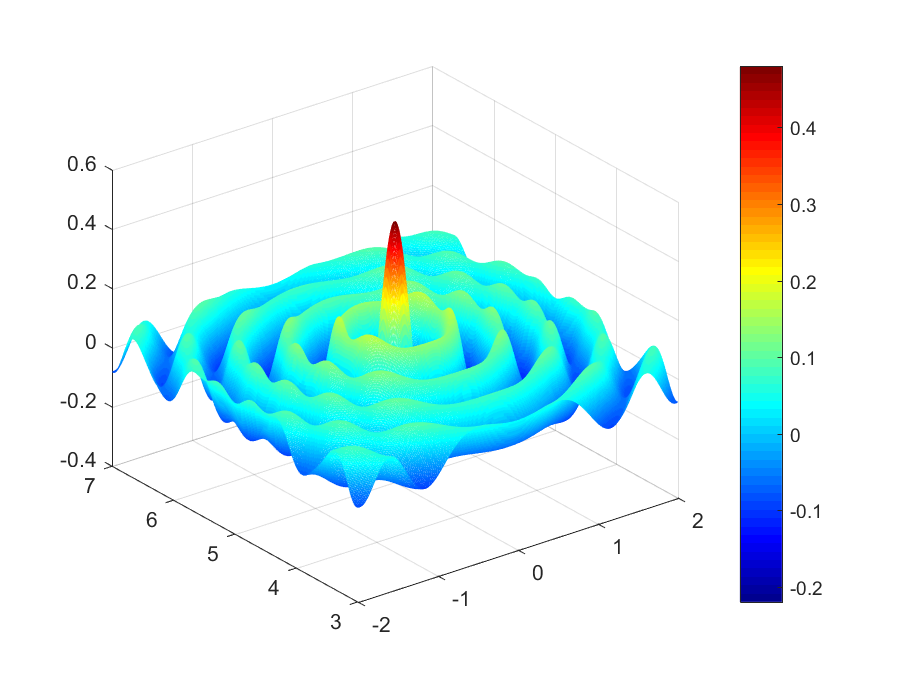
\includegraphics[width=0.8\textwidth]{./intro/psf_chha.eps}
  \caption{$-\Im J(z,y)$,其中$k=4\pi,y=(0,5),z\in[-2,2]\times[3,7]$}\label{fig_psf_chha}
\end{figure}

点扩散函数$J(z,y)$具有如下性质:当$z=y$时,$-\Im J(z,y)$会取得峰值;当$z$逐渐远离$y$点时,$-\Im J(z,y)$会逐渐衰减,具体表现如图\ref{fig_psf_chha}所示。根据文献\cite{ch_ha}中的分析可知,正是由于点扩散函数$J(z,y)$具备如此的性质,才使得成像函数$I_{\rm RTM}(z)$ 对障碍物能够有效成像。受此启发,我们在求解Pekeris开波导障碍物成像问题时,同样可以从点扩散函数出发来选择合适的反传播函数,进而确定适用于Pekeris开波导逆散射问题的逆时偏移算法,详细内容将在第三章和第四章进行讨论。

\section{波导模型初步介绍}
在地球物理反问题当中,被探测的目标大多是嵌入在分层介质当中的,故而近年来以分层介质为背景模型的散射问题和逆散射问题引起了极大地关注。与均匀介质不同,介质的层状结构使得波的传播和散射问题研究变得极为复杂,尤其是波导现象的出现。这导致与之相应的障碍物成像问题也变得较为棘手,很多数值重构算法无法直接加以推广。在本节中,我们将简要地介绍平板声波闭波导和Pekeris开波导模型。

\subsection{平板声波闭波导}
与半空间模型不同,平板声波闭波导除边界$\Gamma_0=\{(x_1,x_2)^T:x_1\in\R,x_2=0\}$之外,还有一个边界$\Gamma_h=\{(x_1,x_2)^T:x_1\in\R,x_2=h\}$。两个边界之间的区域记为$\R^2_h=\{(x_1,x_2)^T:x_1\in\R,x_2\in(0,h)\}$,其被称为波导区域。在波导区域中,时谐声波总场满足Hemholtz方程,且在边界$\Gamma_0$和$\Gamma_h$上分别满足Dirichlet 和Neumann 边界条件,
\begin{eqnarray}\label{cwg}
\left\{
\begin{array}{lll}
   \Delta_x u(x,x_s)+k^2u(x,x_s)=-\delta_{x_s}(x),& in&\R^2_h\backslash\overline{D}\\
   & &\\
   u(x,x_s)=0,& on&\Gamma_0\\
   & &\\
   \frac{\partial u(x,x_s)}{\partial x_2}=0,& on&\Gamma_h\\
   & &\\
   \frac{\partial u(x,x_s)}{\partial\nu}+\i k\eta(x)u(x,x_s)=0,& on&\Gamma_D
\end{array}
\right.
\end{eqnarray}
其中$D$为阻尼系数为$\eta(x)$的阻抗障碍物。类似地,我们可以定义其他边界类型的障碍物和可穿障碍物散射方程。

为保证方程\eqref{cwg}具有物理意义解的唯一性,还需要为其添加合适的辐射条件。设障碍物$D\subset B_R:=(-R,R)\times(0,h)$,其中$R>0$,则由分离变量法可知$u_{x_s}(x_1,x_2):=u(x,x_s)$具有如下模式展开表达式:
\begin{equation}
  u_{x_s}(x_1,x_2)=\sum\limits_{n=1}^{\infty}u_n(x_1)\sin(\mu_nx_2),\ \ \forall |x_1|>R
\end{equation}
其中$u_n(x_1),n=1,2,\cdots,$ 为模式展开系数函数,其满足如下1D的Hemholtz方程:
\begin{equation}\label{cwg_mec}
  u''_n+\xi^2_nu_n=0,\ \ \forall |x_1|>R,\ \ n=1,2,\cdots,
\end{equation}
和辐射条件
\begin{equation}\label{cwg_rad}
 \lim\limits_{|x_1|\rightarrow+\infty}\left(\frac{\partial u_n}{\partial|x_1|}-\i\xi_nu_n\right)=0,\ \ n=1,2\cdots,
\end{equation}
其中,$\mu_n=\frac{2n-1}{2h}\pi,n=1,2,\cdots,$为闭波导模型的截断频率,以及
\begin{eqnarray}
 \xi_n=\left\{
\begin{array}{lll}
   \sqrt{k^2-\mu_n^2}&,&\mu_n<k\\
   \sqrt{\mu_n^2-k^2}&,&\mu_n>k
\end{array}
\right.
\ \ \ n=1,2,\cdots,
\end{eqnarray}
此外,在闭波导模型中,我们总假设波数不等于截断频率,即
\begin{equation}
  k\neq\frac{2n-1}{2h}\pi,n=1,2,\cdots.
\end{equation}

辐射条件\eqref{cwg_rad}保证了1维Hemholtz方程\eqref{cwg_mec}的唯一性,且方程\eqref{cwg}联合辐射条件\eqref{cwg_rad}构成了
闭波导阻抗障碍物散射问题。关于该闭波导散射问题的适定性的研究的文献还有很多,例如
Arens\cite{Arens2010Variational,Arens2011Direct},Morgenr$\ddot{o}$ther\cite{K1988On,K2010on}和 Yongzhi Xu\cite{Xu1990The}。闭波导模型适定性分析的主要困难在于陷阱模式(Embedded Trapped Modes)的存在破坏了散射问题的唯一性,具体分析可见文献\cite{Linton2013Embedded}。当障碍物为如方程\eqref{cwg}中所示的阻抗障碍物时,文献\cite{ch_cw}证明了散射问题的唯一性,并通过极限吸收原理完成了存在性的证明。若障碍物为其他边界类型,由于陷阱模式(Embedded Trapped Modes)的存在,闭波导障碍物散射问题的唯一性并不一定能够得到保证。

\subsection{Pekeris开波导}

在1948年,Pekeris首次提出了半空间两层介质的开波导模型,故而我们称其为Pekeris开波导模型。设$c_0(x)$ 为背景介质速度:
\begin{eqnarray*}
c_0(x)=\left\{
 \begin{array}{lll}
   c_1&,&x\in L_1\\
   c_2&,&x\in L_2
 \end{array}
\right.
\end{eqnarray*}
其中$L_1=\{(x_1,x_2)\in\R^2;x_1\in\R,x_2\in(0,h)\}$表示第一层介质,$h$为第一层介质的厚度,$L_2=\{(x_1,x_2)\in\R^2;x_1\in\R,x_2\in(h,\infty)\}$表示第二层介质。当$c_1=c_2$时,该模型退化为一般的半空间情形;当$c_1>c_2$时,该模型不会产生波导现象;当$c_1<c_2$时,该模型才会产生波导,故而在本文我们仅考虑$c_1<c_2$的情形。令$\Gamma_0=\{(x_1,x_2)^T:x_1\in\R,x_2=0\}$依旧表示半空间的边界,而$\Gamma_h=\{(x_1,x_2)^T:x_1\in\R,x_2=h\}$表示两层介质的
分界面,第一层$L_1$表示波导区域。以可穿透障碍物散射问题为例,类似于半空间均匀背景介质情形,声波波场$u(x,x_s)$满足如下Hemholtz方程和边界条件:
\begin{eqnarray}
 \Delta u(x,x_s)+k^2(x)n(x)u(x,x_s)=-\delta_{x_s}(x),&in&\R^2_+   \label{into_q1_1}\\
 \frac{\partial u(x,x_s)}{\partial x_2}=0,&on&\Gamma_0  \label{into_q1_2}
\end{eqnarray}
其中$\omega$仍表示频率,$c(x)$仍表示波在介质中的传播速度,折射系数$n(x)=\frac{c_0^2(x)}{c^2(x)}$,以及波数$k(x)=\frac{\omega}{c_0(x)}$,即:
\begin{eqnarray*}
k(x)=\left\{
 \begin{array}{lll}
   k_1&,&x\in L_1\\
   k_2&,&x\in L_2
 \end{array}
\right.
\end{eqnarray*}
其中$k_1=\frac{\omega}{c_1},k_2=\frac{\omega}{c_2}$。 易知$k_1>k_2$, 这保证了波导现象的产生。
除此之外,$u(x,x_s)$在分界面$\Gamma_h$处还需满足如下连续性条件:
\begin{eqnarray}
 \left[u(\cdot,x_s)\right]_{\Gamma_h}=0,\ \ \left[\frac{\partial u(\cdot,x_s)}{\partial\nu}\right]_{\Gamma_h}=0 \label{into_q1_3}
\end{eqnarray}

设$u^i(x,x_s)$为点源在$x_s$处激发产生的入射场,则$u^i(x,x_s)=N(x,x_s)$,其中$N(x,y)$为点源在
y处激发而产生的Pekeris开波导Neumann零边界格林函数,它满足如下方程:
\begin{eqnarray}
\left\{
\begin{array}{lll}
  \Delta_xN(x,y)+k^2(x)N(x,y)=-\delta_y(x),&in&\R^2_+\\
  & &\\
  \left[N(\cdot,y)\right]_{\Gamma_h}=0,\ \ \left[\frac{\partial N(\cdot,y)}{\partial\nu}\right]_{\Gamma_h}=0 & &\\
  & &\\
  \frac{\partial N(x,y)}{\partial x_2}=0, &on&\Gamma_0
\end{array}
\right.
\end{eqnarray}
于是散射场$u^s(x,x_s)=u(x,x_s)-u^i(x,x_s)$满足如下方程:
\begin{eqnarray}
\left\{
\begin{array}{lll}
 \Delta u^s(x,x_s)+k^2(x)u^s(x,x_s)=k^2[1-n(x)]u(x,x_s),&in&\R^2_+   \label{into_q3_1}\\
 & &\\
 \frac{\partial u^s(x,x_s)}{\partial x_2}=0,&on&\Gamma_0  \label{into_q3_2}\\
 & &\\
 \left[u^s(\cdot,x_s)\right]_{\Gamma_h}=0,\ \ \left[\frac{\partial u^s(\cdot,x_s)}{\partial\nu}\right]_{\Gamma_h}=0 \label{into_q3_3}
\end{array}
\right.
\end{eqnarray}

类似地,我们可以定义Pekeris开波导不可穿透障碍物散射问题,总场$u(x,x_s)$满足如下方程
\begin{eqnarray}
\left\{
\begin{array}{lll}
 \Delta u(x,x_s)+k^2u(x,x_s)=-\delta_{x_s}(x),&in&\R^2_+\backslash\overline{D}   \label{into_q4_1}\\
 & &\\
 \frac{\partial u(x,x_s)}{\partial x_2}=0,&on&\Gamma_0  \label{into_q4_2}\\
 & &\\
 \left[u(\cdot,x_s)\right]_{\Gamma_h}=0,\ \ \left[\frac{\partial u(\cdot,x_s)}{\partial\nu}\right]_{\Gamma_h}=0 \label{into_q4_3}
\end{array}
\right.
\end{eqnarray}
以及分别针对声软,声硬和阻抗障碍物的三种边界条件:
\begin{eqnarray}
 u=0,\ \ \frac{\partial u}{\partial\nu}=0,\ \ \frac{\partial u}{\partial\nu}+\i k(x)\eta(x)u=0,&on&\Gamma_D
\end{eqnarray}

开波导模型具有广泛的应用价值,故而引起了很多应用数学家的关注和研究,并提出了很多辐射条件以保证开波导散射问题的唯一性和存在性。例如文献Ciraolo和Magnanini\cite{Ciraolo2009A1,Ciraolo2009A2},Bonnet-Ben
Dhia和Christophe Hazard\cite{Dhia2009DIFFRACTION},以及Nedelec\cite{Jerez2012Asymptotics}。类似于闭波导情形,开波导模型同样会产生波导模式和衰减项,辐射条件需要对这两种模式分别进行考虑。与闭波导不同的是,开波导横向和纵向都可以趋于无穷远,而波在这两个方向的传播性质完全不同,故而开波导的分析比闭波导要复杂的多。有意思的是,开波导模型并不会出现类似于闭波导模型下的陷阱模式(Embedded Trapped Modes),该结论的证明可以参考文献\cite{Littman1982Spectral,Weder1988Absence,Hazard2014On}。


我们将在本文第三章以Pekeris开波导模型为例对开波导散射问题和逆散射问题进一步探讨和研究。
而且我们更关心的是如何提出高效准确的数值重构算法,以解决Pekeris开波导模型障碍物成像问题,也就是如下问题:
\begin{question}
 如何通过测量到的散射数据$u^s(x,x_s)$,建立快速有效的数值重构算法,确定嵌入在开波导结构中的障碍物$D$的大小、位置和形状。
\end{question}

如果一个障碍物$D$嵌入在波导结构中,那么想要确定其位置、大小和形状,则会因为波导模式的影响而远比均匀背景介质模型要棘手。关于闭波导逆散射问题的研究已经有很多成熟的算法,例如Arens\cite{Arens2011Direct}和Zhiming Chen
\cite{ch_cw}。对于开波导逆散射问题,也有一些研究结果,例如Robert Gilbert\cite{Gilbert2007Inverse}在一定假设下证明了可穿透障碍物逆散射问题的唯一性;Habib Ammari\cite{Ammari2005Reconstruction}提出了MUSIC 型算法,当障碍物的尺寸比较小时,该算法能够较好确定其位置;Gang Bao\cite{Bao2013Reconstruction}同样对开波导障碍物成像问题的唯一性进行了研究,其唯一性结论需要采集多个频率的远场数据,此外他们还计划将文献
\cite{Bao2005Inverse,Bao2010Error,Bao2011An}中提到的逐步线性化方法推广到开波导模型。

文献\cite{ch_cw}针对平板声波闭波导障碍物成像问题提出了闭波导逆时偏移算法,本文计划将其推广到Pekeris开波导情形,并分析和讨论闭波导和开波导模型有何区别,以及由此而产生的一些有意思的问题和现象。

\newpage
\section{本文主要工作}

本文主要研究了一般半空间以及半空间分层介质上障碍物成像问题的逆时偏移成像算法。文章具体内容安排如下:

第二章主要研究一般的声波半空间障碍物成像问题,在文献\cite{ch_ha}中半空间声波逆时偏移算法的基础上,提出了一种新型的直接成像算法。该算法不需要利用散射场的相位数据信息,仅仅使用总场的振幅数据即可对障碍物进行成像。与此同时,该算法不需要提前知道障碍物的任何先验信息,例如障碍物是否可穿透,以及不可穿透障碍物的边界条件。然后我们通过对新算法成像函数的分辨率分析,证明了在一些合理的假设下,新算法可以达到和半空间逆时偏移算法相同的分辨率。最后,大量的数值算例验证了新算法对障碍物成像的有效性和对噪音的抗干扰性。

第三章主要以Pekeris开波导模型为例对半空间分层介质上的散射问题和逆散射问题进行研究和讨论。首先,我们对Pekeris开波导散射问题进行了简要的介绍;然后,通过对开波导点扩散函数的分析和测试,提出了求解Pekeris开波导模型障碍物成像问题的开波导逆时偏移算法;最后,大量的数值算例表明,开波导逆时偏移算法传承了一般半空间逆时偏移算法的优点,在不需要障碍物任何先验信息的前提下,能够对嵌入在开波导不同介质层的扩展障碍物进行有效成像。特别地,由于反传播函数和开波导模型本身都会产生波导模式,因此开波导逆时偏移算法的分辨率分析要远比一般半空间情形复杂,同时我们也发现了波导模型所特有的一些有意思的问题和现象。


第四章我们对开波导障碍物成像问题继续进行讨论。为解决开波导逆时偏移算法成像函数的收敛性问题,我们首先推导了半空间两层介质Impedance零边界格林函数,并发现当阻抗系数$\lambda$取值适当时,该函数不会产生波导模式。然后通过对点扩散函数的分析和测试,我们提出了阻抗型Pekeris开波导逆时偏移算法。大量的数值算例表明Impedance零边界格林函数可以替代开波导Dirichlet零边界格林函数做为反传播函数。

最后在第五章,我们进行了简单地总结和展望,并指出开波导散射问题和逆散射问题还有很多尚未解决的难题,例如散射问题的高效数值求解算法和逆时偏移算法的分辨率分析,这也是我们下一步将要进行的工作。

